\newpage
\section{Problem 5.8}
\subsection{重要参数}
\begin{align}
f({x_1},{x_2})=&-9{x_1}-10{x_2}\nonumber\\
&-\mu \big[\ln(-{x_1}-{x_2}+100)+\ln (-{x_1}+{x_2}+50)+\ln ({x_1})+\ln ({x_2})\big]
\nonumber
\end{align}


\begin{align}
\bm{g}(x_1, x_2) &= \nabla f(x_1, x_2)\nonumber\\
&=
\begin{bmatrix}
-9 -\dfrac{\mu}{x_1 }+\dfrac{\mu}{100 - x_1 - x_2} + \dfrac{\mu}{50 - x_1 + x_2} \nonumber\\
-10 - \dfrac{\mu}{x_2 }+\dfrac{\mu}{100 - x_1 - x_2} - \dfrac{\mu}{50 - x_1 + x_2}
\end{bmatrix}\nonumber\\\nonumber
\end{align}
\begin{align}
&\bm{G}[x_1, x_2] \nonumber\\
=& \nabla \bm{g}(x_1, x_2)\nonumber \\
=&
\begin{bmatrix}
\dfrac{1}{{x_1}^2 }+\dfrac{1}{(100 - x_1 - x_2)^2} + \dfrac{1}{(50 - x_1 + x_2)^2} 
&\dfrac{1}{(100 - x_1 - x_2)^2} - \dfrac{1}{(50 - x_1 + x_2)^2}\\
\dfrac{1}{(100 - x_1 - x_2)^2} - \dfrac{1}{(50 - x_1 + x_2)^2}&
\dfrac{1}{{x_2}^2 }+\dfrac{1}{(100 - x_1 - x_2)^2} + \dfrac{1}{(50 - x_1 + x_2)^2} 
\end{bmatrix}\nonumber\\ \nonumber
\end{align}

\subsection{算法伪代码}
\begin{algorithm}[h]  
\caption{Backtracking-Armijo Line Search} 
\label{Amj} 
\begin{algorithmic}[1]  
\STATE Choose $\bar{\alpha}>0,\quad \gamma,\rho\in (0,1)$
\STATE Set $\alpha=\bar{\alpha}$
\WHILE {$\phi(\alpha)>\phi(0)+\rho\phi'(0)\alpha$}
\STATE Set $\alpha=\gamma\alpha$
\ENDWHILE
\RETURN $\alpha$ as $\alpha_k$
\end{algorithmic}  
\end{algorithm}

\begin{algorithm}[h]  
\caption{Newton method without Armijo Line Searchfor problem(5.8)}  
\begin{algorithmic}[1]  
\STATE Given $\bm{x}^{(0)}$ and compute $\bm{g}(\bm{x})= \nabla f(\bm{x})$
\STATE Compute $\bm{G}(\bm{x})= \nabla {\bm{g}(\bm{x})}^T$
\STATE Set $\bm{g}^{(0)}=\bm{g}(\bm{x}^{(0)}),k=0$
\WHILE {$\|\bm{g}^{(k)}\|_2>\epsilon$}
\STATE Set $\bm{s}^{(k)}=-{\bm{G}^{(k)}}^{-1}\bm{g}^{(k)}$
\STATE Set $\bm{x}^{(k+1)}=\bm{x}^{(k)}+\bm{s}^{(k)}$
\STATE Set k=k+1
\ENDWHILE
\end{algorithmic}  
\end{algorithm} 

\begin{algorithm}[h]  
\caption{Newton method with Armijo Line Searchfor problem(5.58)}  
\label{NewtonAmj} 
\begin{algorithmic}[1]  
\STATE Given $\bm{x}^{(0)}$ and compute $\bm{g}(\bm{x})= \nabla f(\bm{x})$
\STATE Compute $\bm{G}(\bm{x})= \nabla {\bm{g}(\bm{x})}^T$
\STATE Set $\bm{g}^{(0)}=\bm{g}(\bm{x}^{(0)}),k=0$
\WHILE {$\|\bm{g}^{(k)}\|_2>\epsilon$}
\STATE Set $\bm{s}^{(k)}=-{\bm{G}^{(k)}}^{-1}\bm{g}^{(k)}$
\STATE Compute $\alpha_k$ by Line Search(\textbf{Algorithm} \ref{Amj})
\STATE Set $\bm{x}^{(k+1)}=\bm{x}^{(k)}+\alpha_k\bm{s}^{(k)}$
\STATE Set k=k+1
\ENDWHILE
\end{algorithmic}  
\end{algorithm} 



\subsection{迭代点运动轨迹展示}
\begin{figure}[H]
\centering
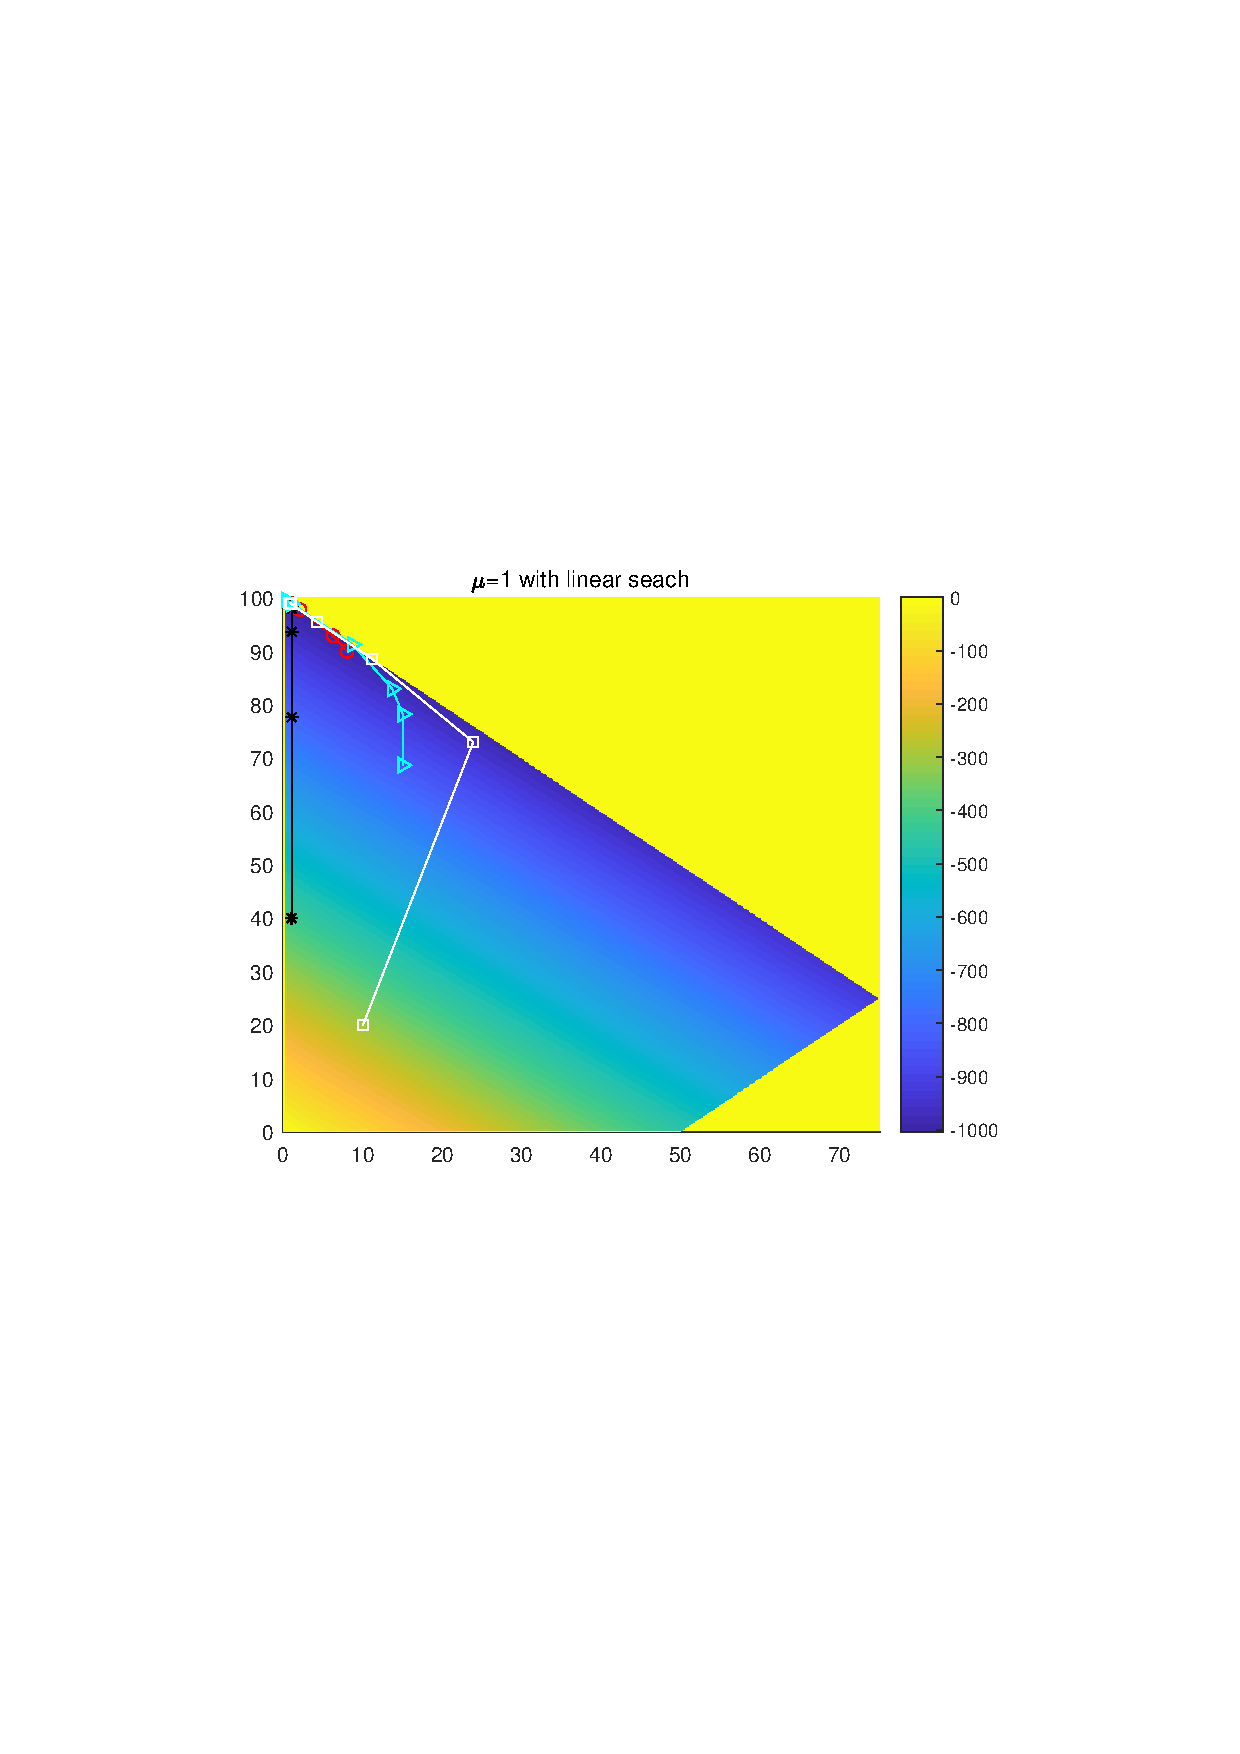
\includegraphics[width=11cm]{fig/5_1.pdf}
\end{figure}

\begin{figure}[H]
\centering
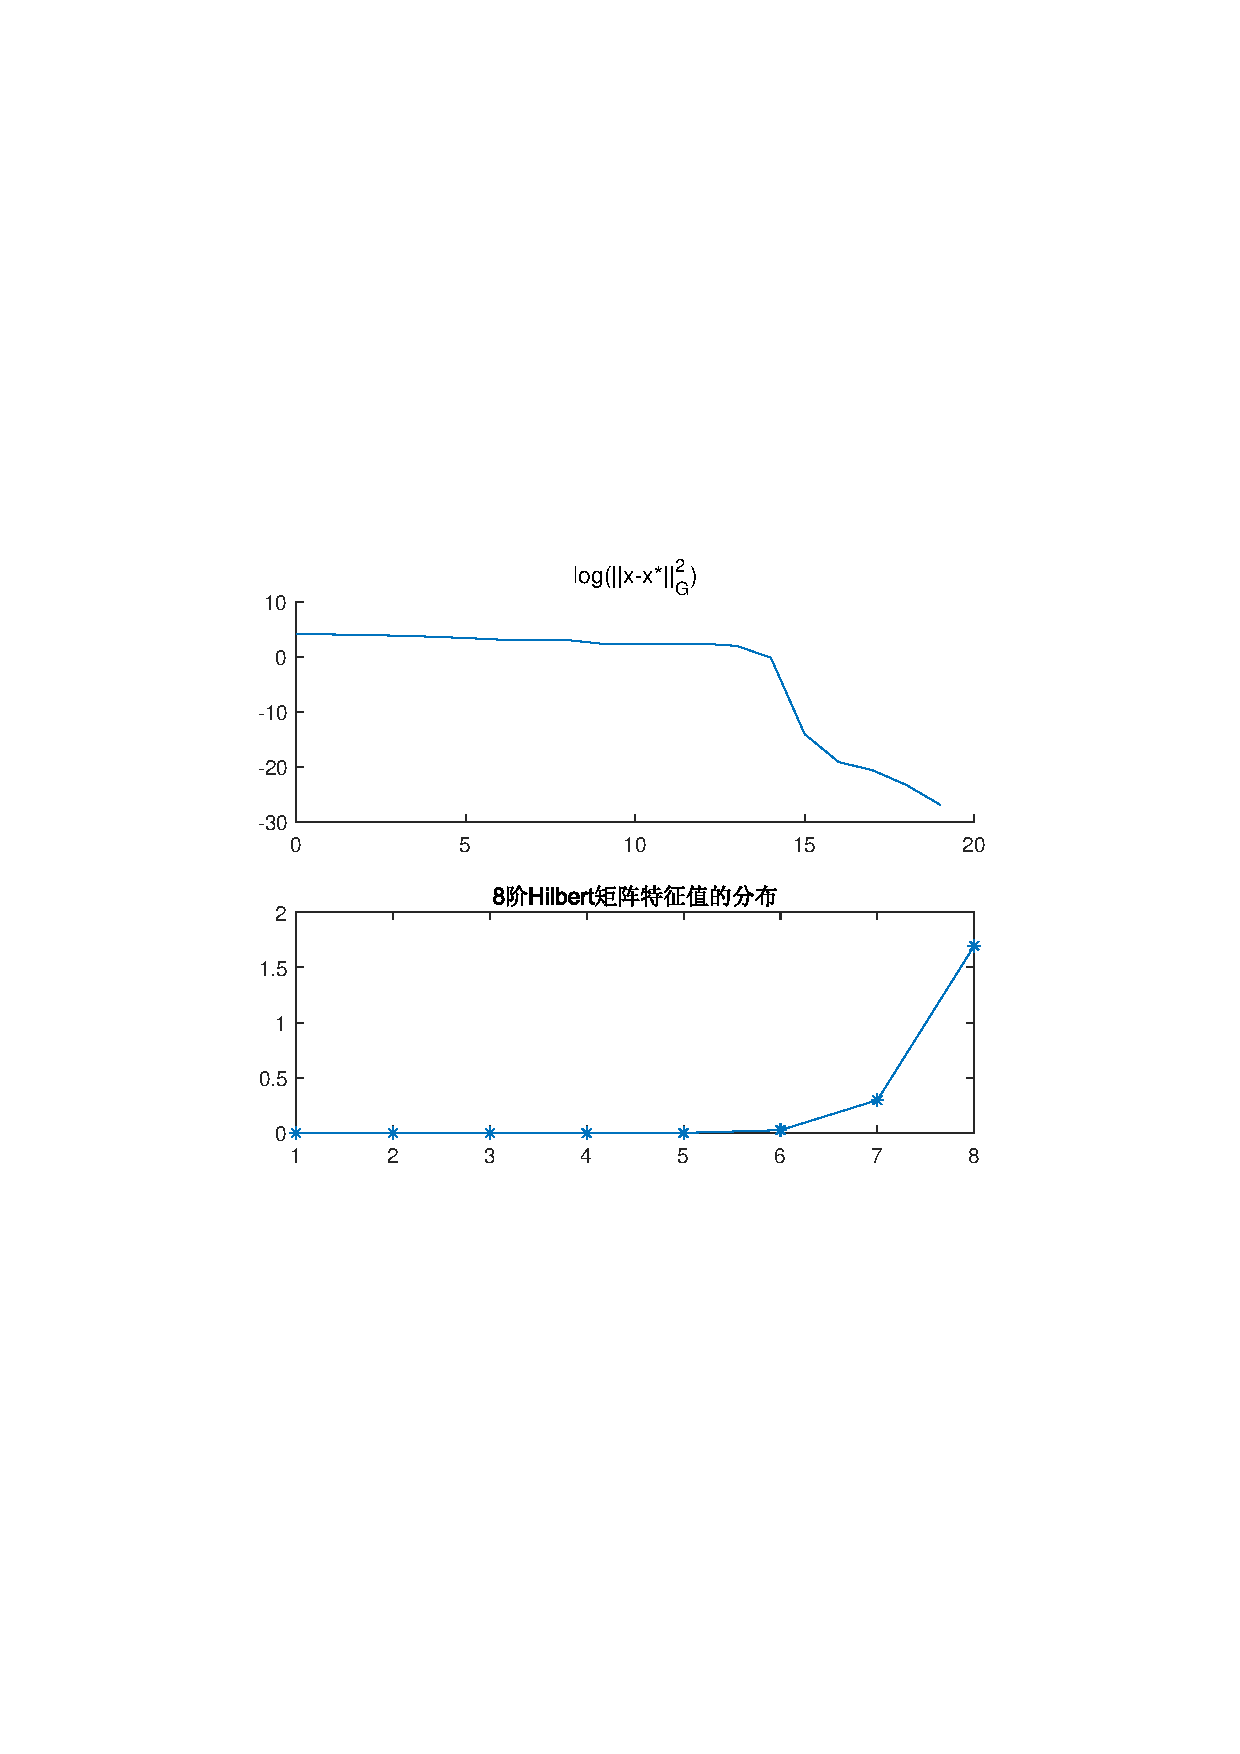
\includegraphics[width=11cm]{fig/5_2.pdf}
\end{figure}

\subsection{总结分析}
本题中Armijo线搜索的参数为$\gamma=0.5,\rho=0.01$

没加线搜索和越界判定之前,牛顿法总是一两次就冲到了定义域外,然后无法收敛。

然后我加了个越界判定:若下一步的迭代点不在定义域内,则将步长$\alpha$缩小一半,牛顿法很好地收敛到了全局最优点。

\begin{lstlisting}
%Check函数检查是否越界,以缩短步长ak
while(Check(x+ak*double(p')))
	ak=0.5*ak;
	xk=x+ak*double(p');
end
\end{lstlisting}

而后在越界判定的基础上加了个线搜索:

\begin{lstlisting}
%采用Armijo法则计算近似步长ak
while(F(xk(1),xk(2)) > (F(x(1),x(2))+0.01*double(p'*g)*ak)
||Check(x+ak*double(p')))%Check函数检查是否越界
	ak=0.5*ak;
	xk=x+ak*double(p');
end
\end{lstlisting}

然而得到的结果与加上线搜索之前一样,可见在迭代的前期,越界判定起到了一定类似于线搜索缩短步长的效果,而到了迭代的后期,牛顿法的基本步长已经满足Armijo法则,还原成了基本牛顿法。

\subsection{牛顿法总结分析}
在面临梯度变化特别大的情况时,最速下降法显得非常不尽人意,即使在离稳定点非常近的地方依旧不能快速收敛,呈锯齿状,由我们所学的知识可以知道,最速下降法的收敛速度强烈依赖于Hessian矩阵的条件数。

而牛顿法显得更加智能
